\documentclass{article}
\usepackage{amsmath, amsfonts, amsthm, amssymb}

\usepackage{bigfoot}
\usepackage{secdot}
\usepackage{epsfig}
\usepackage[T1]{fontenc}
\usepackage{epstopdf}
\usepackage{url}
\usepackage{rotating}
\usepackage{graphicx}
\usepackage{caption}
\usepackage{subcaption}
\usepackage{multirow}
\usepackage{setspace}
\usepackage{array}
\usepackage{fancyhdr}
\usepackage{lastpage}
\usepackage[T1]{fontenc}
\usepackage{xcolor}
\usepackage{multicol}

\usepackage{geometry}
\geometry{letterpaper, left=1in, right=1in, top=1in, bottom=1in}

\pagestyle{fancy}
\fancyhf{}
\rhead{\thepage/\pageref{LastPage}}
\lhead{OSU ECEN 4243 - Computer Architecture - Spring 2023}
\rfoot{\LaTeX}

% ----- Identifying Information -----------------------------------------------
\newcommand{\myassignment}{Using Vivado and the DSDB FPGA}
\newcommand{\myinstructor}{Instructor: Alex Underwood/James E. Stine, Jr.}
\newcommand{\mytas}{TAs: Ross Thompson \\ Ryan Swann \\ Brett Mathis}
% -----------------------------------------------------------------------------

\begin{document}
\begin{center}
  {\huge \myassignment} \\
  \begin{flushright}
    \myinstructor \\
    \mytas \\
  \end{flushright}
\end{center}

This document will explain how to start using Xilinx Vivado to get Lab 0
working on the National Instrument (NI) Digital System Development
Board's (DSDB's) FPGA~\cite{dsdb1}.  The steps listed here will also work for
future labs with some small caveats related to connection of devices
on the DSBB in which implementation on the FPGA will also be required.

\section{DSDB FPGA : Zynq XC7Z020-1CLG484C}

The DSDB has a plethora of devices on it including the main chip we
will use this semester, the Xilinx Zynq FPGA.  The Xilinx Zynq
XC7Z020-1CLG484C is extremely powerful sporting  $650$ MHz
dual-core Cortex-A9 processors,  DDR3 memory controller with $8$ DMA
channels,  high-bandwidth peripheral controllers: 1G Ethernet, SDIO,
and many others.  More information on the DSDB can be found here:
\url{https://reference.digilentinc.com/dsdb/rm} and on Canvas.

All Zynq devices have the same basic architecture, and all of them
contain, as the basis of
the processing system, a dual-core ARM Cortex-A9 processor. This is a
‘hard’ processor (PS) and
it exists as a dedicated and optimized silicon element on the device.
The second principal part of the Zynq architecture is the programmable
logic (PL). This is
based on the Artix\textsuperscript{\textregistered}-$7$ and
Kintex\textsuperscript{\textregistered}-$7$ FPGA fabric.
The PL is predominantly composed of general purpose FPGA logic fabric,
which is composed of slices and Configurable Logic Blocks (CLBs), as
well as Input/Output Blocks (IOBs) for interfacing 
(i.e., these are all Xilinx-specific terms).   As explained in class,
the CLBs are small, regular groupings of logic
elements that are laid out in a two-dimensional array on the PL, and
connected to
other similar resources via programmable interconnects.
Each CLB is positioned
next to a switch matrix and contains two logic slices.  Although
today's FPGAs contain more devices other than CLBS (e.g., Block RAM),
we will primarily use the CLBs for our designs.  These collection of
devices on the FPGAs are typically called System on Chip or SoC devices.

\section{FPGA Implementation}

To start using the Zynq, you will need to use the Vivado EDA toolset
from Xilinx.  Again, just reiterating that you should have your design
working completley in ModelSim simulation before you even attempt an
implementaiton.  You are asking for failure if you decide to proceed
without a good working simulation.

\textbf{Again, please do not begin working through these steps until
  your ModelSim  
  simulations are fully passing to the best of your knowledge.
  Also, make sure you understand the process of verification using a
  testbench with SystemVerilog as it is crucial to getting your FPGA
  implementation working.  Fundamental issues
  with your design will be harder to diagnose and fix if you try to do so in
  Vivado and on the FPGA compared to using ModelSim and running
  simulations.}

Vivado is an extremely powerful EDA tool that can be run in ENDV 360
laboratories.  You can also download and install it on your machines
at home, but it probably does not benefit you much unless you want to
learn more about it.  The Student Edition of ModelSim is the only EDA
tool you will need on your laptop.

\subsection{Vivado System Design}

One of the major factors in modern systems design is the potential for design reuse and
rapid development. Time to market is critical in many application areas, and design tools
that accelerate the development process, crucially without compromising the robustness of
the verification stage or quality of results, bring clear advantages.

The Vivado design flow is based on these principles, and is built on the premise that
many system building blocks are exactly that — ready pieces of
Intellectual Property (IP) that can be integrated
into a project. Unlike older design methods, which typically cater to building systems
entirely from the ground up, Vivado focuses instead on exploiting the pre-verified IP
available in the Vivado libraries (i.e. cores developed by Xilinx), third party IP developers,
or designs by the designer. To a large extent, the focus
of the task has shifted upwards to system integration, rather than low-level hardware
design and the features of the Vivado Design Suite reflect this. Having said that, there is
also the possibility of adding your own logic, which is what we we
will be doing with our Zynq FPGA.  However, we will be using as much
IP in the Vivado system to make sure things work correctly and
interface to your DSDB.

\section{Setting Up the Vivado Project for the First Time}

There is a `Getting Started' zip file on Canvas that contains a pre-made Vivado
project and a \verb|setup.tcl| script that we will use to quickly set up the
project so you can see your ARM single cycle processor in action.  The default
program that the project is set to load into your processor is the 
\verb|memfile.dat| program, but you can change that later~\footnote{I
am calling the output of our compiling process that generates the
\verb!.memfile! the \verb!memfile.dat!.  They are all ASCII files and
can called whatever you want.  Apologies in advance for any ambiguity.}.

\begin{enumerate}
\item Download the repository from GitHub and your Vivado project
  should be inside the \verb|lab2/lab2| subdirectory.  Place the
  \verb|setup.tcl| file on the desktop.  Place the Lab 2 project folder wherever
is convenient for you.

\item Place your \verb|riscv_single.sv| file on the desktop.

\textbf{It is important that both the \texttt{setup.tcl} and
\texttt{riscv\_single.sv} files are on the desktop, as the \texttt{setup.tcl}
script will look for files on the desktop.}

\item Open the Vivado project by first opening Vivado and then clicking Open
  Project under Quick Start (i.e., Figure~\ref{fig:openproject}).
  The Vivado project should be available in your lab2 repository directory.
  Navigate to the Lab 2 project folder
  you extracted from you Canvas zip file and select the Lab 2 project file inside
that folder.
\begin{figure}[h!]
  \centering
  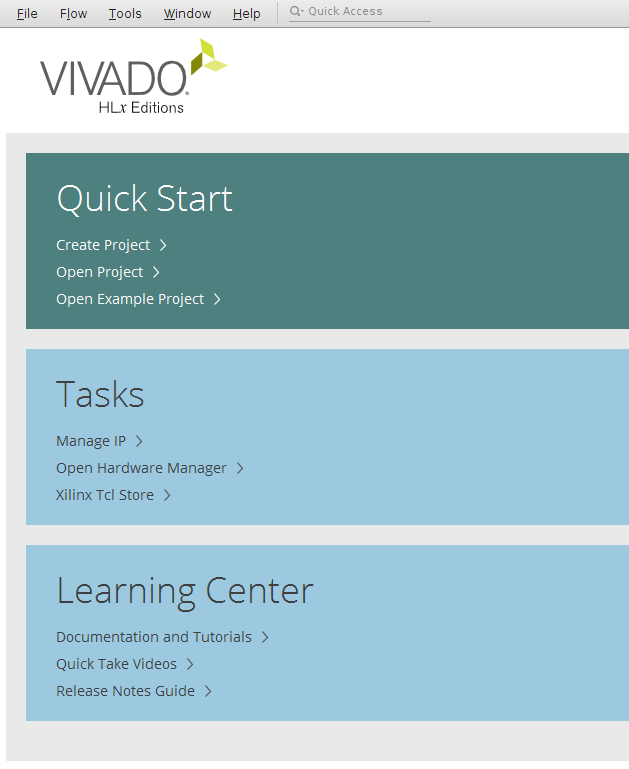
\includegraphics[width=0.4\linewidth]{open_project}
  \caption{Quick Start and Open Project}
  \label{fig:openproject}
\end{figure}

\item Along the bottom of the screen, there is a collection of tabs for various
status views.  Select Tcl Console, which is where we will run our
script (i.e., Figure~\ref{fig:tclconsole}).
\begin{figure}[h!]
  \centering
  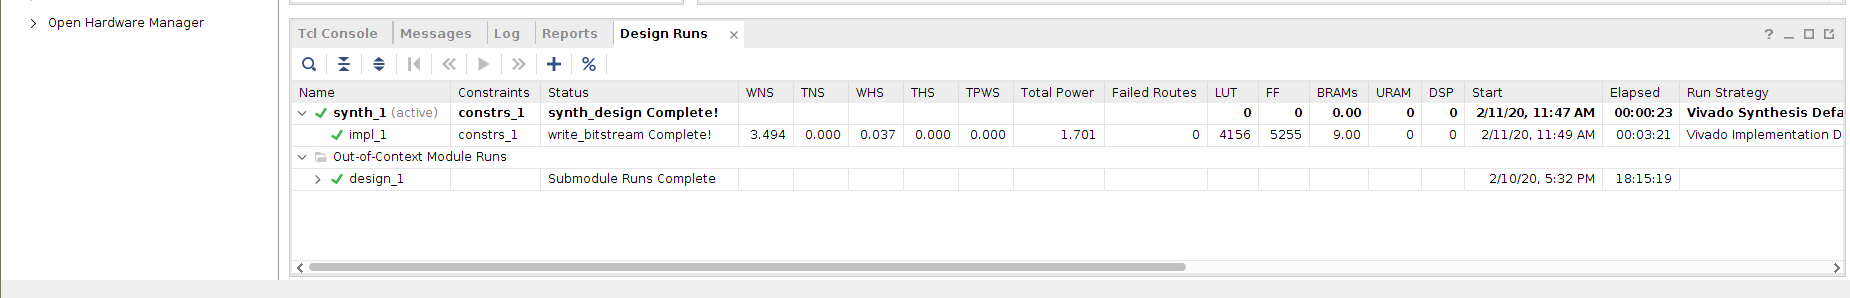
\includegraphics[width=1\linewidth]{tcl_console}
  \caption{Bottom Panel with Tcl Console, Messages, etc.}
  \label{fig:tclconsole}
\end{figure}

The Tcl Console behaves much like a terminal or command prompt in which you can
run commands through keyboard entry instead of using the mouse and GUI.  This
allows us to script some of the more complex components involved in setting up
a project and skip to the more important parts for this class including testing
and profiling your design.

Just like a terminal, the Tcl Console runs inside a specific directory, but you
can change that directory using the \verb|cd| command.  First, use the command
\verb|pwd| to Print your Working Directory (where you currently are).  Using
that information, Navigate to your desktop by typing \verb|cd ..| to
ascend a folder level and \verb|cd <name of folder>| to descend into that
folder.  Your goal here is to navigate to the desktop where we put the
\verb|setup.tcl| and \verb|riscv_single.sv| files.

\item Once on the desktop, run the following command in the Tcl Console:

\verb|source setup.tcl|

\verb|source| is the command used in Tcl to run a script stored in a file. This
script will do the following things:
\begin{itemize}
\item Search your desktop for the \verb|top_module.sv| file and copy that
  file into the project directory.
	
\item Refresh the project index, causing the modules that connect to the
  RISC-V core to see the newly added file and update their references.
	
\item Clean up the project to clear away any lingering errors or warnings
  regarding Block Generation, Synthesis, or Implementation.
	
\item Beginning running the project toolchain which will start with Block
  Generation in which each top level module in the project will be
  synthesized to check for usability.  Then, Synthesis will convert the entire
  design and all surrounding components into a netlist
  that represents real hardware.  Following that, Implementation will convert
  the hardware netlist into a design the FPGA can understand.  Finally,
  Generate Bitstream will create a file that can be uploaded to the FPGA and
  allow the FPGA to start using your design.
\end{itemize}
All of these steps are automatic when you run the script and will chain into
each other so long as no errors occur during any steps.  \textbf{Again, this is
why you do not want to start using the FPGA until your simulation works - errors
here take longer to find and are often more complicated to solve than if you had
found them in your simulations in ModelSim.}  These steps might take some time to
run (approximately 5 minutes) - you can view their progress in the Design Runs
tab on Figure~\ref{fig:tclconsole}

If you run into errors or issues here, go to the Messages tab
in Figure~\ref{fig:tclconsole} where messages, warnings, and errors are stored and see
what happened, or delve even deeper in the Log tab where the output from the
toolchain is directly stored.

If you need to make modifications to your files,
you will need to do so in Vivado now because \textbf{the script will copy the
file on your desktop into the project directory}.  Modifications made to the
file on your desktop will not be reflected in the project.  Go to Open Block
Design on the left panel and then select the Sources tab in the upper left
window (i.e., Figure~\ref{fig:sources}).  You'll have to do a bit of digging through
the source tree to get to
your RISC-V core because this project has many components in the background to make
things run, expand the design\_1\_wrapper, design\_1, top\_0,
design\_1\_top\_0\_0, and finally inst : top to reveal your RISC-V core called
\verb|riscvsingle:riscvsingle|.  Double-click that entry to open the file.  Make your changes
and save the file.
\begin{figure}[h!]
  \centering
  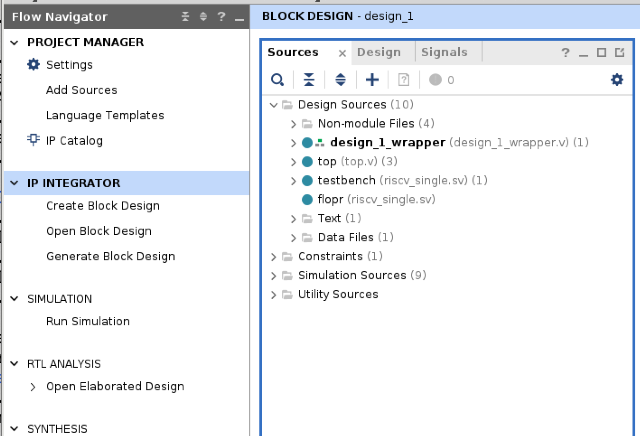
\includegraphics[width=0.7\linewidth]{sources2}
  \caption{Open Block Design and Sources Window}
  \label{fig:sources}
\end{figure}

Anytime you make a change to the file and save it, a message will appear along
the top of the screen that the Module References are Out-of-Date
(i.e., Figure~\ref{fig:refreshmodules}).  Like what the
script was doing, you've changed the module, but the other modules that connect
to the RISC-V core haven't had a chance to refresh themselves and update their
references.  Clicking Refresh Changed Modules on that message will update the
project index and refresh all references.  You can then run the toolchain just
like the script did by clicking Generate Bitstream on the bottom-left
panel (i.e., Figure~\ref{fig:generatebitstream}).  A
window will pop up letting you know that Synthesis is out-of-date and that will
need to run first - answer Yes so all required steps will run first.  Then, the
Launch configuration window will open where you can set details about how the
toolchain will run.  Leave these at the defaults and click OK.  Go
to the Design Runs tab in Figure~\ref{fig:tclconsole} to see each step's
progress while waiting for them to complete (approximately 5 minutes).
\begin{figure}[h!]
	\centering
	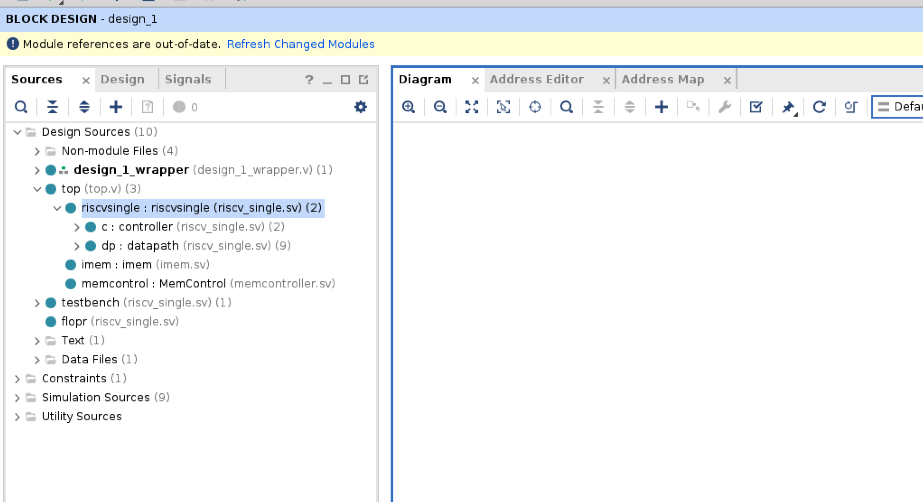
\includegraphics[width=0.9\linewidth]{refresh_modules2}
	\caption{Refresh Changed Modules Banner}
	\label{fig:refreshmodules}
\end{figure}
\begin{figure}[h!]
	\centering
	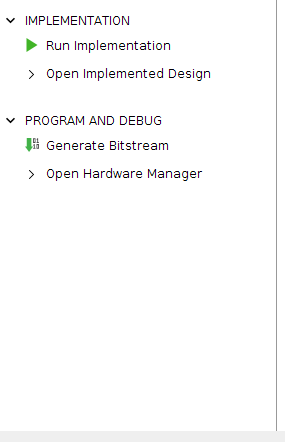
\includegraphics[width=0.3\linewidth]{generate_bitstream}
	\caption{Generate Bitstream under Program and Debug}
	\label{fig:generatebitstream}
\end{figure}

\item Once Bitstream Generation is complete, a window will pop up asking what
you would like to do next (i.e., Figure~\ref{fig:generatebitstream}).  Select Open
Hardware Manager and click OK.  If you accidentally close this window or select
something else, you can easily get to the hardware manager using the Open
Hardware Manager button below Generate Bitstream in
Figure~\ref{fig:generatebitstream}.
\begin{figure}[h!]
	\centering
	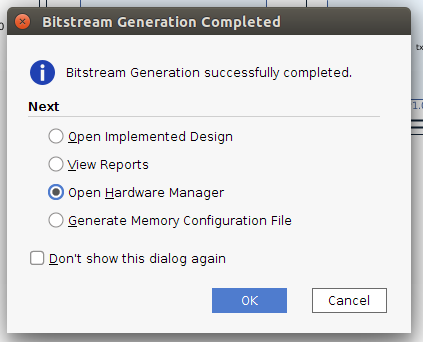
\includegraphics[width=0.4\linewidth]{bitstream_complete}
	\caption{Bitstream Complete, Open Hardware Manager}
	\label{fig:bitstreamcomplete}
\end{figure}

\item If you have not already done so, now is the time to connect your DSDB to
the computer and power it on, as the next step will involve opening a connection
to it in Vivado so you can upload your design to the FPGA.

Remove the prototyping board from the Elvis III at your desk by pulling the
board horizontally towards you.  Connect the DSDB by lining up the gold fingers
along the top of the board with the socket on the top of the Elvis III.  Make
sure the board is laying flat before pushing the board into the socket - the
holes in the PCB along the bottom should slide into the plastic notches along
the bottom of the Elvis III.  Connect the DSDB to the computer at your station
using the microUSB to USB cable included in it's box.

\emph{Yes, even though
the DSDB is connected to the Elvis III, which is itself connected to the
computer already, you still need to connect the DSDB to the computer with the
USB cable in order to interact with the FPGA through Vivado.}

\textbf{The DSDB will be powered by the connector along the top of the board
through the Elvis III - you do not need to power it with another power source.
Do \underline{not} connect a power supply to the barrel connector on the top right of the
DSDB}.

Power on the Elvis III using the power switch along the top-back of the device.
Then, power on the expansion board with the button on the upper left of the
Elvis III.  Finally, make sure the boot switch \verb|SW8| on the DSDB is set to
\verb|QSPI|, and then power on the DSDB with the power switch on the upper
right of the board.  Now your DSDB is powered on and connected to your system.
You can check to make sure you have the correct boot switch setting by flipping
the switches \verb|SW0|-\verb|SW7| on the board, and their corresponding LEDs
\verb|LD0|-\verb|LD7| should light up.

\item With the Hardware Manager open in Vivado and your DSDB connected to the
Elvis III and the computer as well as powered on, click Open Target along the
top banner that alerts you that no hardware target is open, and then click Auto
Connect (i.e., Figure~\ref{fig:opentarget}).  This will automatically search the
system for any powered-on devices that can interface with Vivado and connect to
them for easy programming.
\begin{figure}[h!]
	\centering
	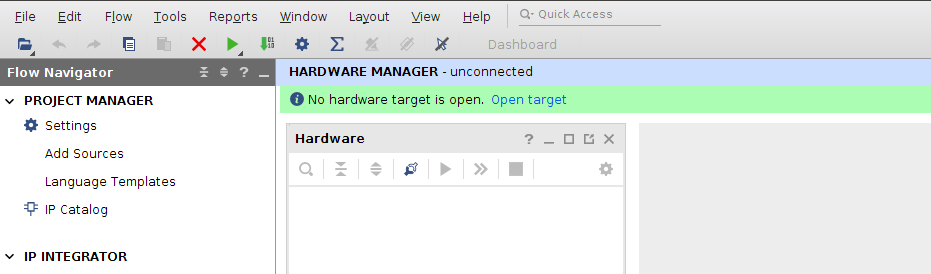
\includegraphics[width=0.8\linewidth]{open_target}
	\caption{Open Hardware Target}
	\label{fig:opentarget}
\end{figure}

\item Once connected, the auto connect banner along the top will change to tell
you there are no debug cores connected.  This isn't an issue - our debug core is
built-in to the design so it will connect once you program the device.  Click
Program device (i.e., Figure~\ref{fig:programdevice}).
\begin{figure}[h!]
	\centering
	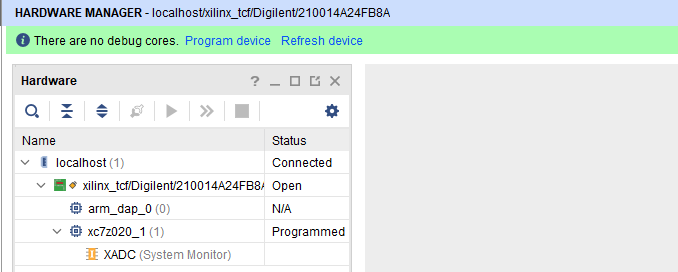
\includegraphics[width=0.8\linewidth]{program_device}
	\caption{Program Device once Connected}
	\label{fig:programdevice}
\end{figure}

\textbf{Starting at this stage and until specified later, you need to press and
hold the bottom-right button \texttt{BTN0} on the DSDB.  This button is bound to
the reset signal in the processor and will keep the processor in a reset state
once it has been programmed.  We want to keep the processor in reset so it
doesn't begin running until we've finished prepping the debug tool that will let
us observe the system as it runs, so continue holding the button down while
programming the device and prepping the debug window.}

After clicking Program device, a window will open in which you get to select the
bitstream and debug profile to upload to the FPGA
(i.e., Figure~\ref{fig:selectbitstream}).  These fields will be auto-populated, so (with
\verb|BTN0| held down), you can click program FPGA. The FPGA will load your
design and the Hardware Manager window will change to look like a signal
analyzer similar to ModelSim.
\begin{figure}[h!]
	\centering
	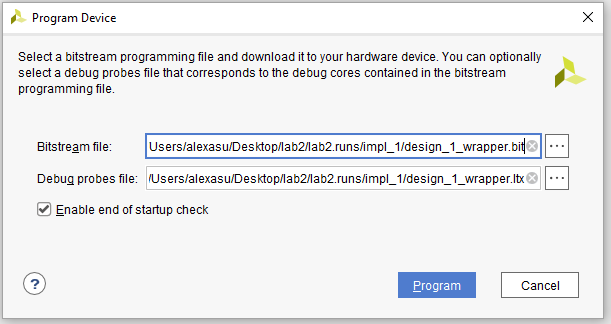
\includegraphics[width=0.8\linewidth]{select_bitstream}
	\caption{Select BitStream and Debug Image to Program}
	\label{fig:selectbitstream}
\end{figure}

\item With the FPGA programmed and \verb|BTN0| still held down, press the play
button along the top panel of the signal analyzer view that has appeared in the
Hardware Manager window to arm a debug trigger that has been
pre-applied (i.e., Figure~\ref{fig:ilawaveform}).
\begin{figure}[h!]
	\centering
	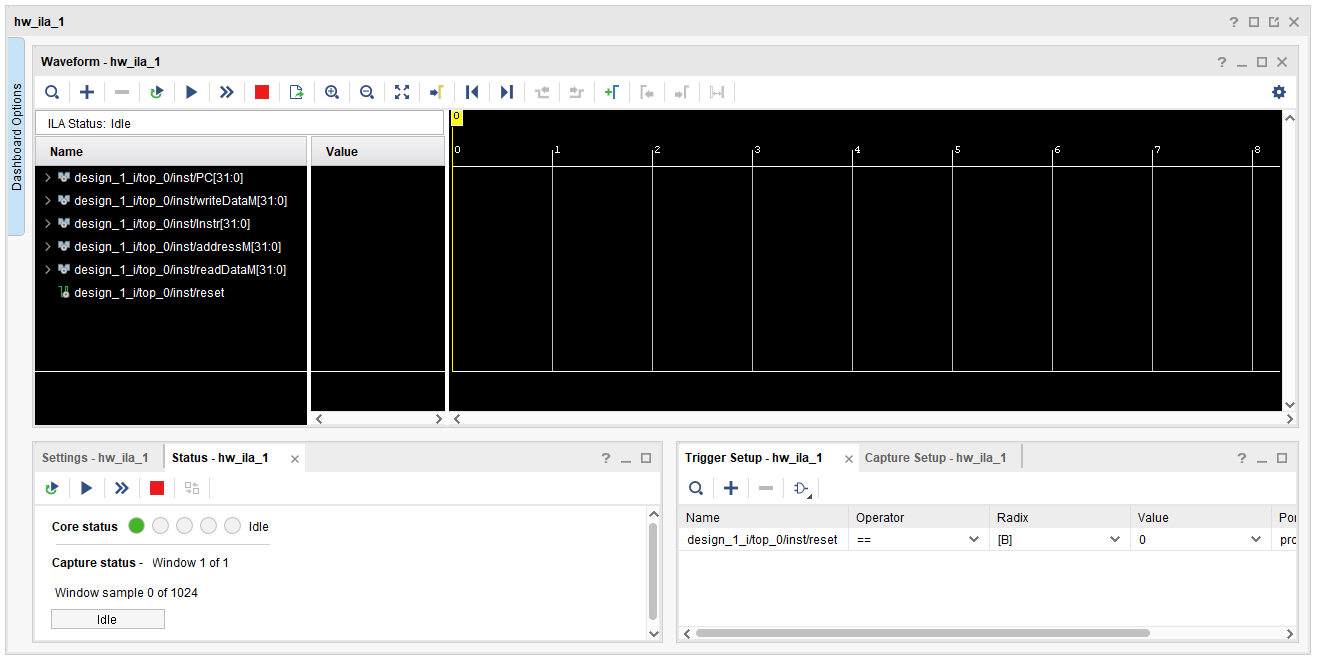
\includegraphics[width=0.9\linewidth]{ila_waveform}
	\caption{Signal Analyzer and Debug Trigger Menus}
	\label{fig:ilawaveform}
\end{figure}

Unlike simulations which can just generate the next value and save that on the
computer, the FPGA is a real system with a real circuit on-board, meaning that
capturing the data inside is a little trickier.  To capture this data, a debug
core has been pre-added to this project that observes some of the data that
flows into and out of your RISC-V core.  But, because these data measurements take
place on the FPGA and then the data is sent back to the computer, only so much
data can be saved at a time.  This is where debug triggers come in - we can set
the debug core to only save data when a certain event takes place such as a
specific signal reaching a specified value or even a Boolean function of
multiple signals.  We have pre-made a trigger for this project to detect when
the reset signal is logic low (which, because you are still holding down
\verb|BTN0|, is currently logic high).  Pressing the play button arms the
trigger so the debug core starts actively cycling through data, waiting to save
the current data it has as soon as the trigger is true.

Once the play button has been pressed and the trigger is armed, release
\verb|BTN0| which will complete the trigger requirements and cause the debug
core to start taking data.  This will simultaneously bring the RISC-V core out of
the reset state and it will begin executing the program it was loaded with (the
default is \verb|memfile.dat|).

The signal analyzer window will populate with data - $512$ data points per signal
before the reset signal went low and $512$ data points per signal after the reset
signal went low.  You can use the values in the signal analyzer window to view
view the performance of your system by matching the value of your RISC-V core's
FPGA with the instruction it should be executing at that point and see as values
pass by on the memory and address busses.

Specifically, we are interested in
the memory performance of the system, so we want to see how long the system is
forced to wait for \verb|LW| and \verb|SW| operations to complete.
\verb|fib.s| has both of these operations, but you should test other
programs later as well.  Once you've found a memory operation (fairly easy to
find, as they take the most time when looking at the signal analyzer view),
calculate how many cycles they take by positioning the cursor (click and drag
it) at the end of the operation to get the exact end time, then position the
cursor at the start of the operation to get the exact start time.  Subtract
start time from end time and that will be your memory response time for this
particular program on your RISC-V core.

Remember that load and store both take
different amounts of time, so measure the response time of both.  Of course,
this is also a good opportunity to make sure your RISC-V core is still functional
by seeing if the value read out of memory in the \verb|memfile.dat| program
matches the value that was written to memory just a couple of instructions
prior.  If that isn't working, then your measure of the memory's response time
may not be accurate because the rest of the processor isn't working as intended.

If you re-run the trigger and press reset after you have already captured data
once, the debug core will still capture data and your RISC-V core will still be
functioning, but because the system repeats the same program over and over (the
instruction memory in the FPGA is only as big as it needs to be to hold the
program you specified to load in) the positions used in memory for the program
will already hold the correct values and the values read from memory might still
be on the memory read port due to the small number of \verb|LW| instructions
preventing the value on that port from being overwritten.

You can rerun the program from scratch by powering off the DSDB and then
powering it back on.  Vivado might throw an error because the board was
disconnected without warning, but simply follow the steps to auto-connect to the
board and proceed from there to run a completely fresh run again.
\end{enumerate}

By now, you should have your Vivado project set up so that it contains your
modified and functional \verb|riscv_single.sv| file, the project has run through
the toolchain including Block Generation, Synthesis, Implementation, and finally
Bitstream Generation, and you've been able to upload the bitstream to the FPGA
and see your processor function correctly on the FPGA running the
\verb|memfile.dat| program.  With this, you've been able to take the data on how
long each \verb|LW| and \verb|SW| operation should take when using real memory
like that of the DSDB.

\section{Changing the Program the RISC-V Core will Run}

By default, the project from Canvas will load the \verb|memfile.dat| program.
Once you've successfully run that program on your own RISC-V core on the FPGA, you
should try running some other programs and see what results you get and how they
compare.  The project comes with \verb|memfile.dat| and \verb|fib.s| 
pre-added, making it fairly easy to swap between the two programs.  If you want
to run your own programs, you can do that as well but the section after this one
will cover how to add those files to the project so Vivado knows where to look
for them.

\begin{enumerate}
\item Navigate to the sources view as explained in the previous section under
step~$5$ and shown in Figure~\ref{fig:sources}.  You'll want to descend the source
tree just like it was explained before, but this time open \verb|imem.sv| instead
of \verb|riscv_single.sv|.  Inside this file, you will find the following line:

\verb|initial $readmemh("memfile.dat", RAM);|

This is the command that loads the program into instruction memory.  Changing
\verb|"memfile.dat"| to your respective \verb|"xxx.memfile"| will load in any program
into the FPGA.  Currently, the \verb|"memfile.dat"| should be the
Fibonacci program in the riscvtest directory.

\item Save the changes to the file and follow the steps from the first section
of this guide again starting halfway through step~$5$.  These steps boil down to
the following things:
\begin{itemize}
\item Refresh Changed Modules using the button on the top banner
  (i.e., Figure~\ref{fig:refreshmodules}).
  
\item Generate Bitstream, which will also run all necessary steps prior to
  that in the process and Open Hardware Manager once complete.
  
\item Make sure your DSDB is connected to the computer, set to \verb|QSPI|
  boot, and powered on.
  
\item Auto Connect to hardware target, hold down \verb|BTN0| and program
  the FPGA.
  
\item Arm the trigger in the signal analyzer with the play button, then
  release \verb|BTN0| to begin running the program.
  
\item Take data on the results of the program execution on your hardware.
\end{itemize}
\end{enumerate}
By now, you should have been able to go through the
toolchain in order to upload your design to the FPGA and see it in
action using the debug information.

\section{Adding your own Programs into Vivado}

\begin{figure}[h!]
  \centering
  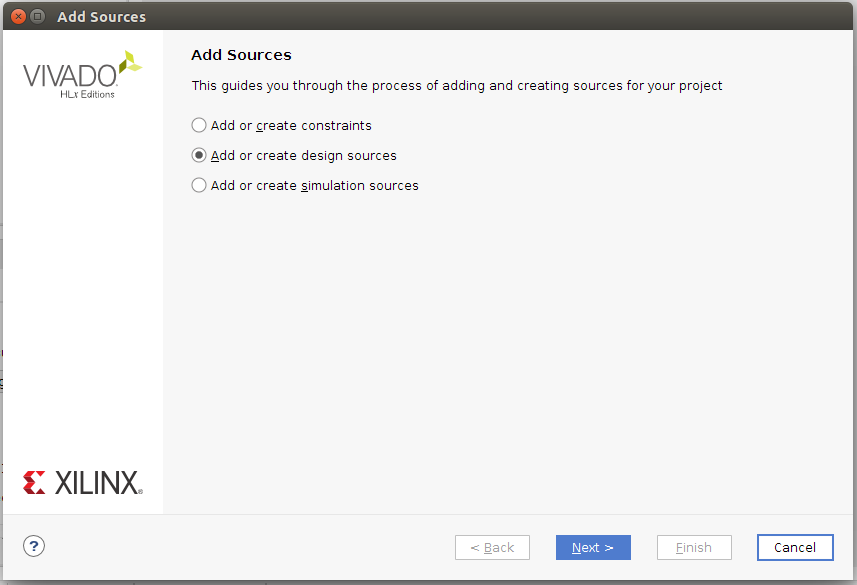
\includegraphics[width=0.8\linewidth]{add_sources}
  \caption{Open Hardware Target}
  \label{fig:addsources}
\end{figure}
\begin{figure}[h!]
  \centering
  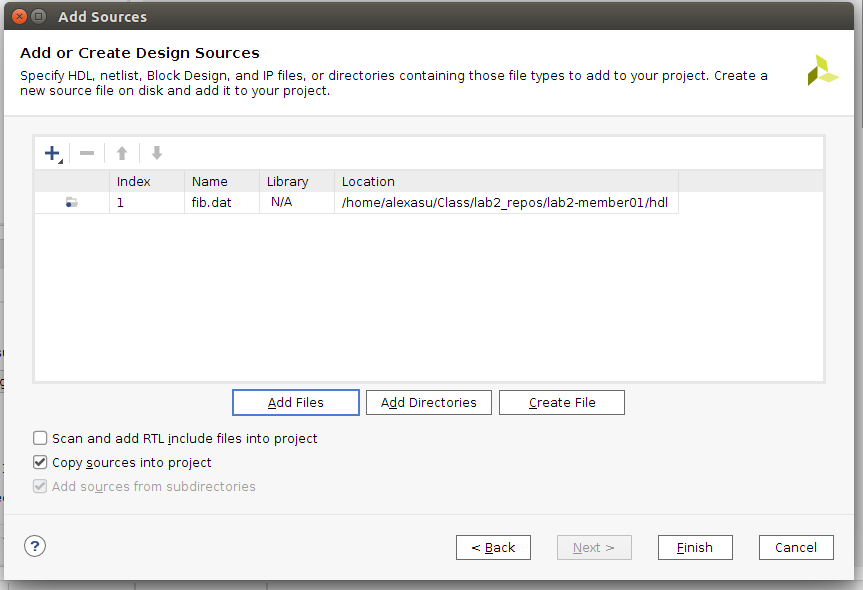
\includegraphics[width=0.8\linewidth]{copy_sources}
  \caption{Open Hardware Target}
  \label{fig:copysources}
\end{figure}
You can run your own programs on your RISC-V core as well.  To do this, you will
need to import the \verb|.dat| file for the program into your Vivado project,
then follow the steps in the previous section on Changing the Program the RISC-V
Core will run to change which program will be loaded into the instruction
memory.  Right now, the instruction memory is hard-coded into the FPGA
within the Block RAM.

\begin{enumerate}
\item Click Add Sources under the Project Manager heading on the left panel
(i.e., Figure~\ref{fig:sources}).

\item Select Add or create design sources on the window that opens and click
Next (i.e., Figure~\ref{fig:addsources}).

\item Select Add Files to open a file browser you can use to navigate to your
\verb|.dat| file.  By default, the file browser will be looking for HDL source
files, so you'll need to change file type visibility by clicking the Files of
Type drop down menu and selecting All Files.  Select your \verb|.dat| file and
click OK.  You can select more than one \verb|.dat| file if you'd like to add
multiple files at the same time.

\item The files you selected will be listed in the Add or Create Design Sources
window.  Make sure the Copy sources into project box is checked and then click
Finish (i.e., Figure~\ref{fig:copysources}).

\item  With the new \verb|.dat| files added to your project, follow the steps in
the previous section to change which \verb|.dat| file will get loaded into the
instruction memory and then continue through the steps to run the toolchain,
upload the bitstream to the FPGA, and test your design.
\end{enumerate}

\bibliographystyle{IEEEtran}
\bibliography{IEEEabrv,fpga_guide}


\end{document}
